\documentclass[a4paper, 11pt]{article}
\usepackage{fullpage} % changes the margin
\setlength\parindent{24pt} % for indenting with \par
\usepackage{sectsty}

\sectionfont{\fontsize{11}{11}\selectfont}

% for inserting image
\usepackage{graphicx}
\graphicspath{}

% listings for inserting code --
\usepackage{color}

\definecolor{dkgreen}{rgb}{0,0.6,0}
\definecolor{gray}{rgb}{0.5,0.5,0.5}
\definecolor{mauve}{rgb}{0.58,0,0.82}


% for bold line under section heading
\usepackage{titlesec}
\titleformat{\section}
  {\normalfont\Large\bfseries}{\thesection}{1em}{}[{\titlerule[0.8pt]}]

%%%%%%%%%%%%%%%%%%%%%%%%%%%%%%%%%% 
\begin{document}
%%%%%%%%%%%%%%%%%%%%%%%%%%%%%%%%%%


\begin{titlepage} % Suppresses headers and footers on the title page

	\centering % Centre everything on the title page
	
	\scshape % Use small caps for all text on the title page
	
	\vspace*{\baselineskip} % White space at the top of the page
	
	%------------------------------------------------
	%	Title
	%------------------------------------------------
	
	\rule{\textwidth}{1.6pt}\vspace*{-\baselineskip}\vspace*{2pt} % Thick horizontal rule
	\rule{\textwidth}{0.4pt} % Thin horizontal rule
	
	\vspace{0.75\baselineskip} % Whitespace above the title
	
	{\LARGE Using Xfinity On Campus:\\} % Title
	\vspace{0.5\baselineskip} % Whitespace below the editor list
  {\scshape How to Use Internet \\ To Access Television}
	
	\vspace{0.75\baselineskip} % Whitespace below the title
	
	\rule{\textwidth}{0.4pt}\vspace*{-\baselineskip}\vspace{3.2pt} % Thin horizontal rule
	\rule{\textwidth}{1.6pt} % Thick horizontal rule
	
	\vspace{2\baselineskip} % Whitespace after the title block
	
	%------------------------------------------------
	%	Subtitle
	%------------------------------------------------
	
	
	\vspace*{3\baselineskip} % Whitespace under the subtitle
	
	%------------------------------------------------
	%	Editor(s)
	%------------------------------------------------
	
	\vspace{0.5\baselineskip} % Whitespace before the editors
	
	\vspace{0.5\baselineskip} % Whitespace below the editor list
	
	{\scshape ResNet \\ 831-459-4638 \\
          10AM - 12PM, 1PM - 5PM, Monday - Friday \\
          Rachel Carson College (formerly College 8)
  } % Editor affiliation
	
	\vfill % Whitespace between editor names and publisher logo
	

\end{titlepage}

%----------------------------------------------------------------------------------------




%%%%%%%%%%%%%%%%%%%%%%%%%%%%%%%%%%
% 1 
%%%%%%%%%%%%%%%%%%%%%%%%%%%%%%%%%%
\section*{
  Connecting to Xfinity On Campus with a computer
}

You can connect to Xfinity On Campus with a computer or other device that
talks to the internet.  From here you may stream on demand, save shows, and 
watch live TV. 

While some televisions may be receiving a functioning cable connection via
a coaxial connection, the full features described will not be 
experienced unless one is connected to an internet connection.\\
{\newline}
\textbf{How to Connect}

In order to connect to Xfinity On Campus you must be connected to one of the
campus networks.  This includes: UCSC-Guest, Eduroam, ResWiFi, or through a 
wired Ethernet connection.\\
{\newline}
\textbf{Logging into Xfinity On Campus}
\begin{itemize}
  \item To connect to Xfinity On Campus from your computer, ensure that your device  is connected to the internet. 
  \item From your browser, navigate to https://www.xfinityoncampus.com/.  Enter University of California Santa Cruz in the 'search for your school' bar.
\end{itemize}
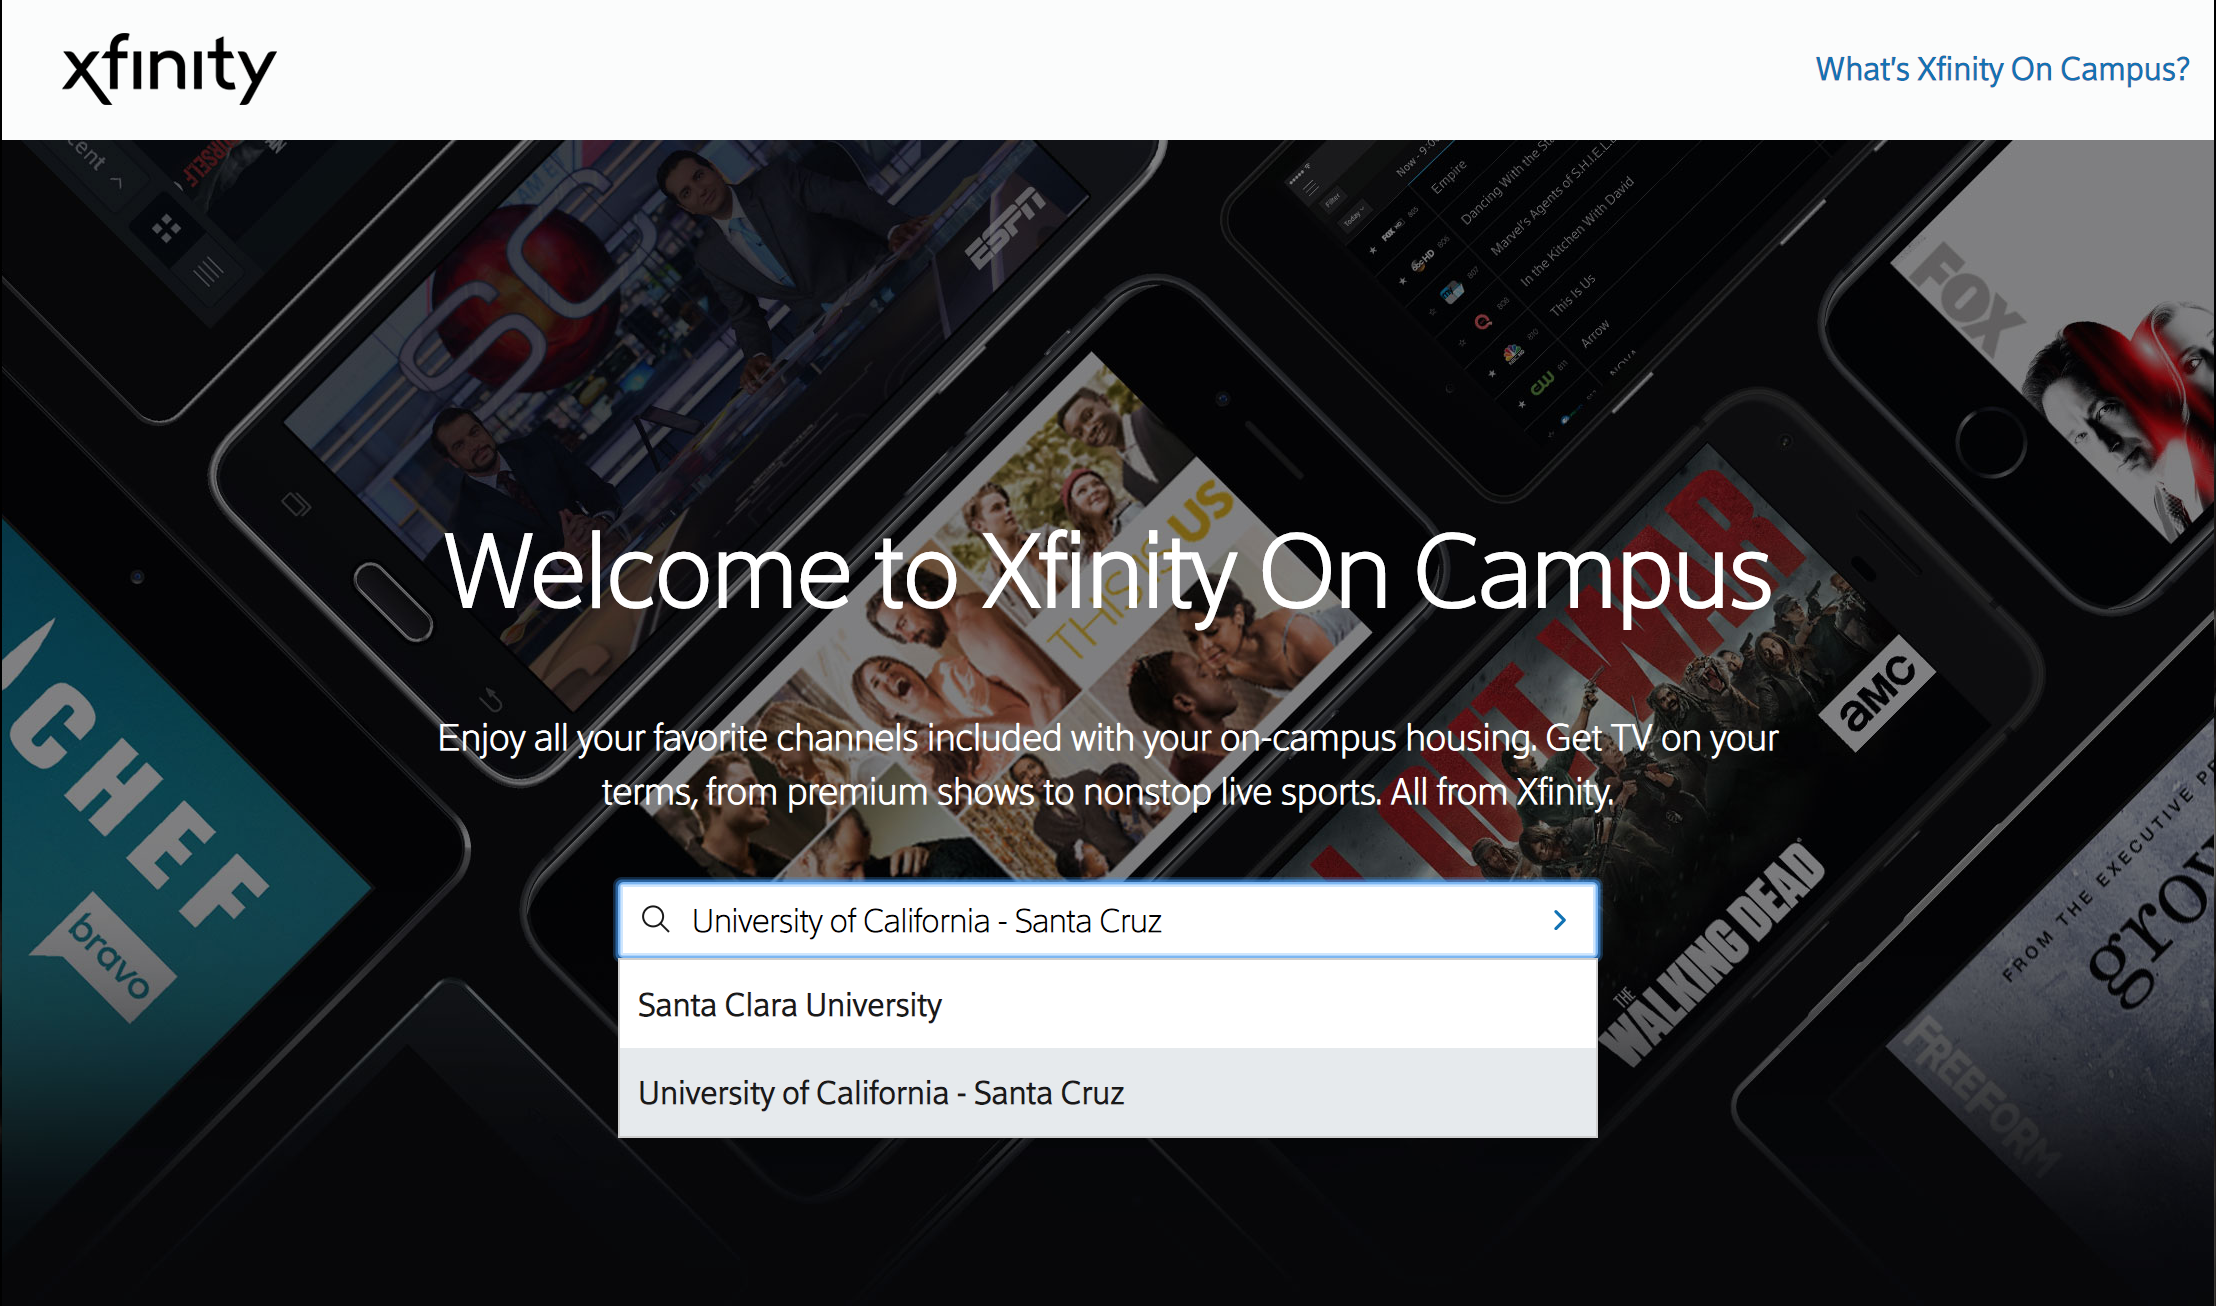
\includegraphics[width=\linewidth, height=\textheight, keepaspectratio]{welcome.png}
\begin{itemize}
  \item enter your cruz credentials, afterwards youll be directed to a new URL
  https://www.xfinity.com/stream/

\end{itemize}
notes:
To use xfinity on campus must be connected via a campus wifi or wired
connection.
While some televisions may be receiving a functioning cable connection via
a coaxial connection, the full features will not be experienced unless one
is connected with an internet connection.

Navigate to https://www.xfinityoncampus.com/
enter University of California Santa Cruz

enter cruzid and gold password on prompt
answer notice of infomration

watch now:
  You will be directed to a new URL https://www.xfinity.com/stream/
  you may have to enable flash in browser
  from here you may:
  browse shows available on demand
  or select Live Tv from the drop down header menu and browse for a desired
  channel.

Channels:
  This will tell you your line up of channels available\
  When connected to the tv may watch this from your television or your computer.  The channels link will still redirect you to the same URL as 
  watch now.


  


\end{document}

